\documentclass[tikz,border=2pt]{standalone}
\usepackage{amsmath,amssymb}
\usepackage{pgfplots}
\pgfplotsset{compat=1.18}
\begin{document}
% On the sample space (0,1) with probability = length and U(u) = u: Y equals U except at u = 1/2,
% where Y = 0, so {Y != U} = {U = 1/2} has probability 0 and Y = U a.s.; 1 - U agrees with U only
% at u = 1/2, so U and 1 - U are almost surely different.
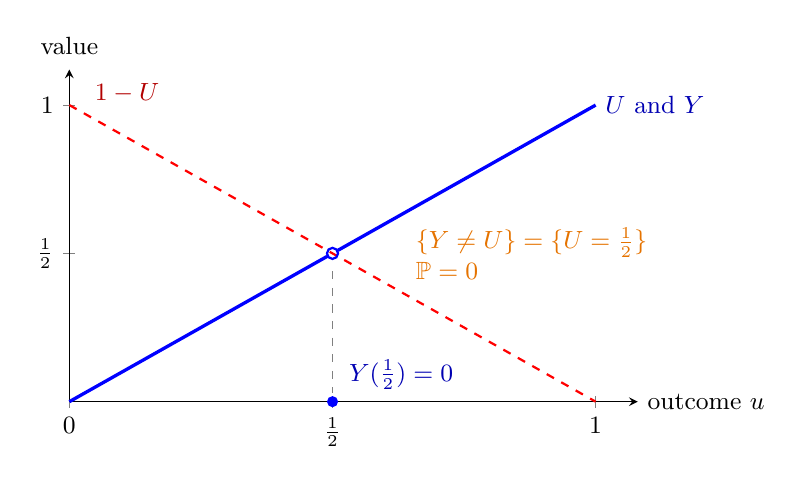
\begin{tikzpicture}[font=\small]
  \begin{axis}[
    axis lines=left,
    xmin=0, xmax=1.08, ymin=0, ymax=1.12,
    xtick={0,0.5,1}, xticklabels={$0$,$\tfrac{1}{2}$,$1$},
    ytick={0.5,1}, yticklabels={$\tfrac{1}{2}$,$1$},
    xlabel={outcome $u$}, ylabel={value},
    xlabel style={at={(axis description cs:1,0)}, anchor=west},
    ylabel style={rotate=-90, at={(axis description cs:0,1)}, anchor=south, yshift=2pt},
    width=8.8cm, height=5.8cm, clip=false
    ]
    % 1 - U, dashed red
    \addplot[red, thick, dashed, domain=0:1] {1-x};
    \node[red!70!black, anchor=west] at (axis cs:0.03,1.04) {$1-U$};
    % Y = U except at 1/2
    \addplot[blue, very thick, domain=0:0.49] {x};
    \addplot[blue, very thick, domain=0.51:1] {x};
    \addplot[only marks, mark=o, mark size=2pt, blue, thick, fill=white] coordinates {(0.5,0.5)};
    \node[blue!70!black, anchor=west] at (axis cs:1.0,1.0) {$U$ and $Y$};
    % the value of Y at the exceptional outcome
    \draw[gray, thin, dashed] (axis cs:0.5,0.44) -- (axis cs:0.5,0.03);
    \fill[blue] (axis cs:0.5,0) circle (2pt);
    \node[blue!70!black, anchor=south west, inner sep=2pt] at (axis cs:0.52,0.02) {$Y(\tfrac{1}{2})=0$};
    \node[orange!90!black, anchor=west, align=left] at (axis cs:0.64,0.5) {$\{Y\neq U\}=\{U=\tfrac{1}{2}\}$\\$\mathbb{P}=0$};
  \end{axis}
\end{tikzpicture}
\end{document}
